\documentclass[a4j, twocolumn]{jarticle}
\usepackage{graphicx}
\usepackage{titling}
\usepackage{subcaption}
\usepackage{caption}
\usepackage{amsmath}

\graphicspath{{./images/}}

\begin{document}
  \title{インドネシア \\\large 東南アジアの隠れた美しさ}
  \author{Christian Harjuno\thanks{釧路工業高等専門学校情報工学科}}
  \date{\today}
  \maketitle
  \section{インドネシアってなんですか?}
  インドネシア, またはインドネシア共和国は, 東南アジアにある国の一つです. 赤道の中央に位置し, インドネシアの列島はシンガポール, マレーシア, オーストラリアの間にあります. 2020年の国勢調査によると, インドネシアの人口は約2億7千万人で, 世界で4番目に多いです. 
  インドネシアについてよく知っている外国の方は少ないと思います. 「インドネシアについて何かご存知ですか」と聞けば, 最も多い答えは「バリ島」ですが, 実際のインドネシアはそれ以上にすばらしい国だと思います. したがって, 今回はインドネシアについてより詳しく説明したいと思います. 
  \section{地理と多様性}
  \subsection{地理}
  前に説明した通り, インドネシアはシンガポール, マレーシア, オーストラリアの間にあり, 面積は約$190.000 km^2$で, インドネシアは世界で14番目に大きな国土面積を持っています. インドネシアは多数の島々を有することで知られており, 周囲を海に囲まれ, 17,508以上の島が存在します\cite{ANDREFOUET2022104848}. 図\ref{indonesiamap}を見ると, インドネシアにはスマトラ島, ジャワ島, カリマンタン島, スラウェシ島, そしてパプア島という本島があります. 各島には全く異なる文化や言語が存在します.\\
  \subsection{人口と民族}
  2020年の国勢調査によると, インドネシアの人口は約2億7,000万人で, 世界で4番目に多いです\cite{unstats2023}. その地理的条件と歴史的背景から, インドネシアには1,331以上の公的に認定された民族集団が存在し, 700以上の言語が国全体にわたって分布しています.\\
  \begin{figure}
    \centering
    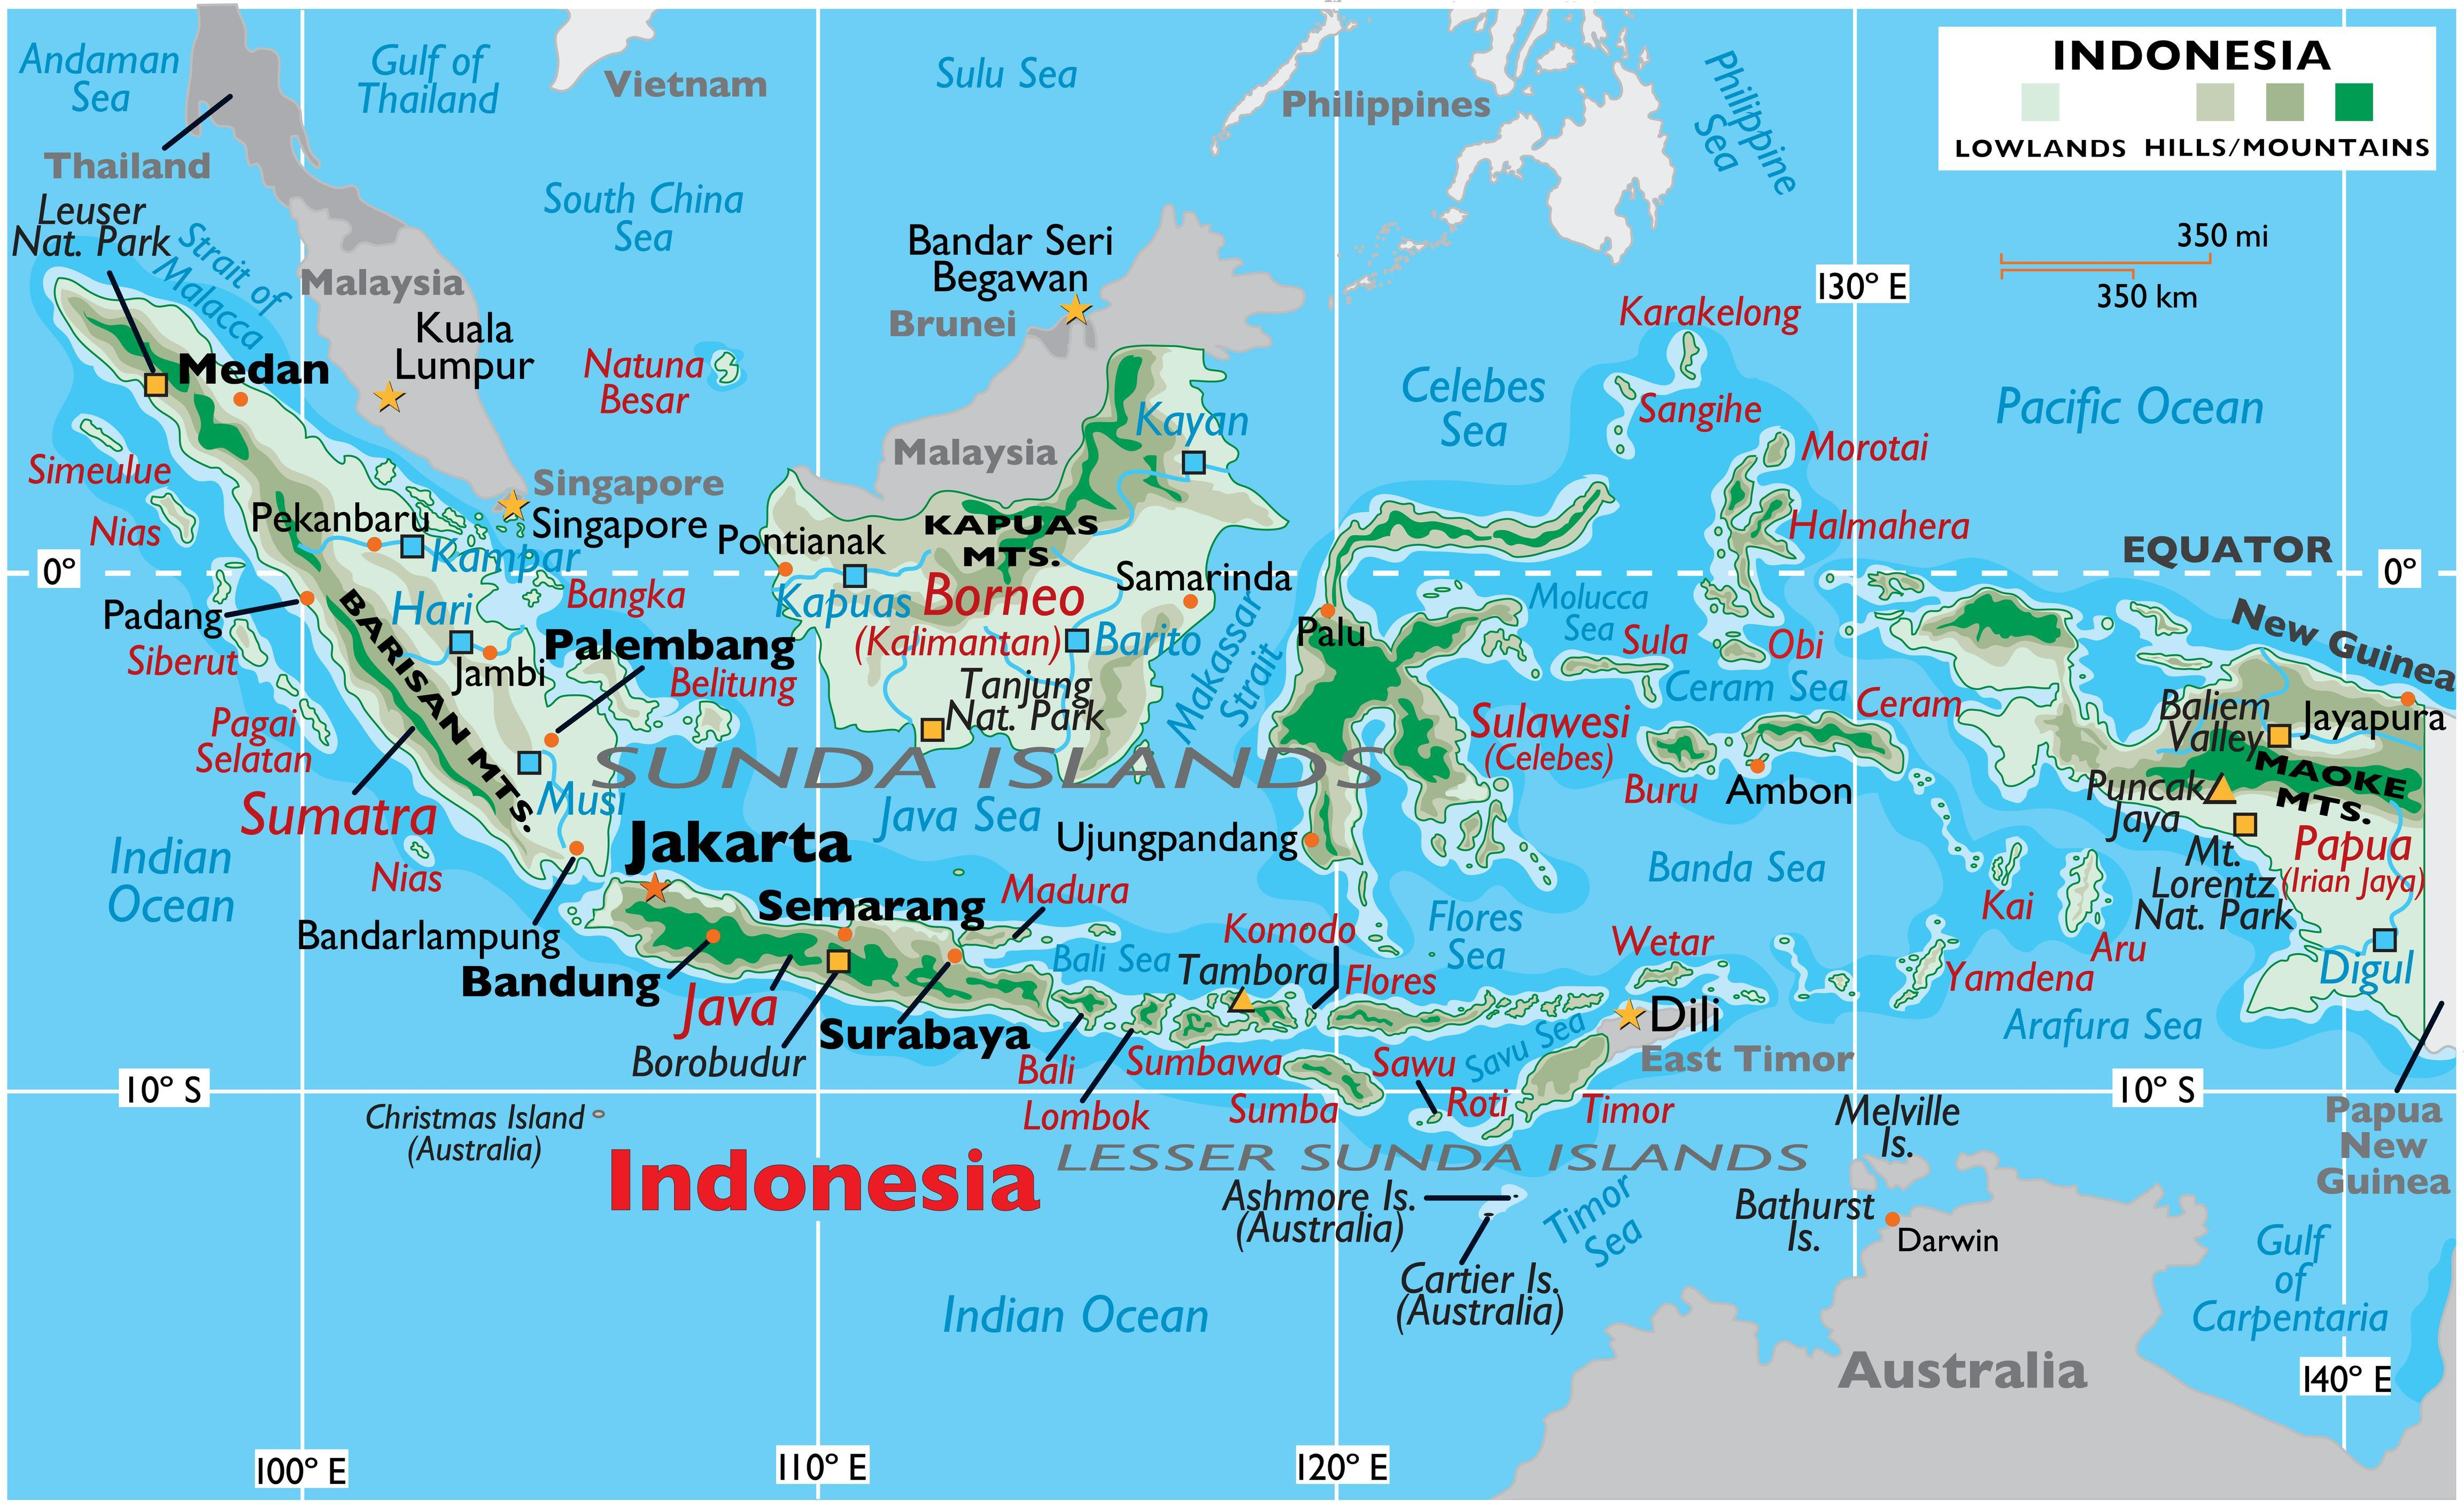
\includegraphics[width=\linewidth]{indonesia-map.eps}
    \caption{インドネシアの地図}\label{indonesiamap}
  \end{figure}
  \begin{figure}
    \centering
    \includegraphics[width=\linewidth]{webber-wallace-line.eps}
    \caption{ウォレスとウェーバーの路線地図}\label{wallaceweber}
  \end{figure}
  \subsection{博物}
  また, 民族だけでなく, インドネシアの動植物も非常に興味深いと思います. 図\ref{wallaceweber}を参考にすると, 1800年代のイギリスの博物学者アルフレッド・ラッセル・ウォレスはインドネシアの列島の中央に線を引き, 動植物の種類を明確に区別しました. ほとんどの動物の種, 特に鳥類は, その線を越えない傾向があります. その線の左側には, アジアでも見られる動物が含まれています. 一方, 右側には, オーストラリアでも見られる動物が含まれています. この線によって分けられているため, インドネシアは豊かな生物多様性を持っています\cite{wallaceline}
  \subsection{宗教}
  インドネシアは歴史的にシャーマニズムの国でしたが, インドの商人たちが岸に到達し, 地元の人々にヒンドゥー教を教えたことで変わりました. ヒンドゥー教がその時期に広まり, ヒンドゥー教の名のもとに新しい王国が興亡を繰り返しました. その後, 仏教がインドネシアの商人たちによって伝わり, 当時最も新しく人気のある宗教となりました. それも, アラビアの商人を通じてイスラム教がシルクロードを経て伝わるまでのことです. イスラム教はインドネシアで急速に広まり, 現在もその影響は続いています\cite{philtar_indonesian_religions}.\\
  \begin{table}[htb]
    \caption{インドネシアにある宗教の比率}\label{religion-percentage}
    \centering
    \begin{tabular}{|c|c|}
      \hline
      宗教 & 人口の割合 \\
      \hline
      イスラム教 & 87.1\% \\
      \hline
      キリスト教 & 10.4\% \\
      \hline
      カトリック教 & 3.12\% \\
      \hline
      仏教 & 0.71\% \\
      \hline
      儒教 & 0.07\% \\
      \hline
      ヒンドゥー教とそのほか & 1.7\% \\
      \hline
    \end{tabular}
  \end{table}
  表\ref{religion-percentage}により, インドネシアの人口の87%がイスラム教徒であり\cite{pew2024indonesia}, 残りはキリスト教, カトリック, 儒教, ヒンドゥー教, 仏教が信仰されています\cite{penpres1965}. 大多数がムスリムであるにもかかわらず, インドネシアは憲法に基づいて宗教の自由を保障しているため, 厳密にはムスリム国家ではありません. インドネシアでイスラム教が大きく広まった後, 大航海時代に入り, イギリスやオランダの貿易商が約300年間にわたってインドネシアを植民地化したことで, カトリックやキリスト教など他の宗教も伝わってきました\cite{philtar_indonesian_religions}.
  \section{歴史}
  インドネシアの歴史は, さまざまな宗教の王国の興亡に大きく彩られています. スリウィジャヤ王国は東南アジアの広範囲を支配し, マジャパヒト王国は現在のインドネシアの大部分を統一したことで知られています\cite{kemdikbud2017sejarahX} (p.100--).\\
  15世紀, ヨーロッパの大航海時代と世界的な香辛料貿易の影響で, ポルトガルの船乗りや商人がインドネシアに到来しました. ポルトガル人の到来は, ヨーロッパ諸国がマレー半島へ進出する新たな道を開きました. 16世紀には, オランダ東インド会社(VOC)がインドネシアを征服し, 約300年間にわたる植民地支配が始まりました\cite{kemdikbud2017sejarahXI} (p.9--).\\
  この300年間には, イギリスやフランスによる支配の変化もあり, インドネシアの人々にとっては一時的な平和も訪れました. しかし, オランダによる統治は苦痛と犠牲を伴うものでした. 厳しい納期や重い課税, 腐敗により, 栄養失調や過労で数百万人が命を落としました\cite{kemdikbud2017sejarahXI} (p.46--).\\
  第二次世界大戦が勃発すると, 日本の帝国陸軍がオランダからインドネシアの支配権を奪いました. 日本の支配はわずか3年間でしたが, 戦争のための資源調達を目的とした過酷な搾取により, オランダの300年に及ぶ支配以上の苦しみをインドネシアにもたらしました\cite{kemdikbud2017sejarahXI} (p.235--). \\
  日本が戦争から撤退した後, インドネシアは1945年8月17日に独立を宣言しました. これは, アメリカ合衆国が日本に原子爆弾を投下してからわずか数日後のことでした\cite{safitry2021sejarah} (p.131--).

  \begin{figure}
    \centering
    \includegraphics[width=\linewidth]{equator.eps}
    \caption{赤道路線地図}\label{equator}
  \end{figure}
  \section{観光と気候}
  \subsection{気候}
  図\ref{equator}の通り, インドネシアは赤道の真ん中に位置しており, 熱帯気候です. 年間を通して平均気温と湿度は非常に高く, 太陽は一年を通して明るく輝き, 日中の平均気温は12度です. この高温多湿の熱帯気候は森林の生育に最適な環境を作り出し, 何百万もの生物にとって最適な生息地となっています. しかし, インドネシアには年間を通して雨季と乾季の2つの季節しかありません\cite{handoyo2021geografi} (p.1--8). \\
  日本と同様に, インドネシアは環太平洋火山帯に位置しています. インドネシアには全国に数百もの活火山があり, 毎日定期的に地震が発生しています\cite{handoyo2021geografi} (p.13).\\
  インドネシアは熱帯気候なので, 一年に四季がある日本と比べて, 気温の変化があまり激しくありません. インドネシアは熱帯気候のため, 一年に四季がある日本と比べて気温の変化はそれほど激しくありません. しかし, インドネシアの地形は起伏に富んでいるため, 場所によって平均気温が異なります\cite{intrepid2023weather}.\\

  加重平均を計算するため, 次の式を利用します. \\
  \begin{equation}
    加重平均 = \frac{\sum_{i=1}^{n} w_i x_i}{\sum_{i=1}^{n} w_i}
  \end{equation}\label{weightedaveragetemperature}
  ここで, 
  \begin{itemize}
    \item \( x_i \):各月の平均気温(値)
    \item \( w_i \):各月の日数(重み)
    \item \( n \):月の数(通常は 12)
  \end{itemize}
  地方によって, 月々の平均温度は異なってるので, 表\ref{baliaveragetemp}によってバリ島のデータを例として計算して見ていきます\cite{intrepid2023weather}. \\
  \begin{table}[h]
    \caption{バリ島の月々の平均温度}\label{baliaveragetemp}
    \centering
    \begin{tabular}{|c|c|c|}
      \hline
      月 & 最高平均温度 & 最低平均温度 \\
      \hline
      3月~5月 & $33^\circ\mathrm{C}$ & $24^\circ\mathrm{C}$ \\
      \hline
      6月~8月 & $30^\circ\mathrm{C}$ & $23^\circ\mathrm{C}$  \\
      \hline
      9月~11月 & $32^\circ\mathrm{C}$ & $23^\circ\mathrm{C}$ \\
      \hline
      12月~2月 & $33^\circ\mathrm{C}$ & $24^\circ\mathrm{C}$ \\
      \hline
    \end{tabular}
  \end{table}
  \begin{equation}\label{baliaveragetempcalculation}
    \begin{aligned}
      年間平均最高気温 = \frac{33 + 30 + 32 + 33}{4} = \frac{128}{4} = 32^\circ\mathrm{C} \\
      年間平均最低気温 = \frac{24 + 23 + 23 + 24}{4} = \frac{94}{4} = 23.5^\circ\mathrm{C}
    \end{aligned}
  \end{equation}
  計算式\ref{weightedaveragetemperature}を利用して, \ref{baliaveragetempcalculation}によると, バリ島の年間的の加重平均温度は最高$32^\circ\mathrm{C}$と最低$23.5^\circ\mathrm{C}$\cite{mendenhall2013introduction}.

  \subsection{観光}
  \begin{figure}[h]
    \centering
    \begin{subfigure}[b]{0.3\textwidth}
      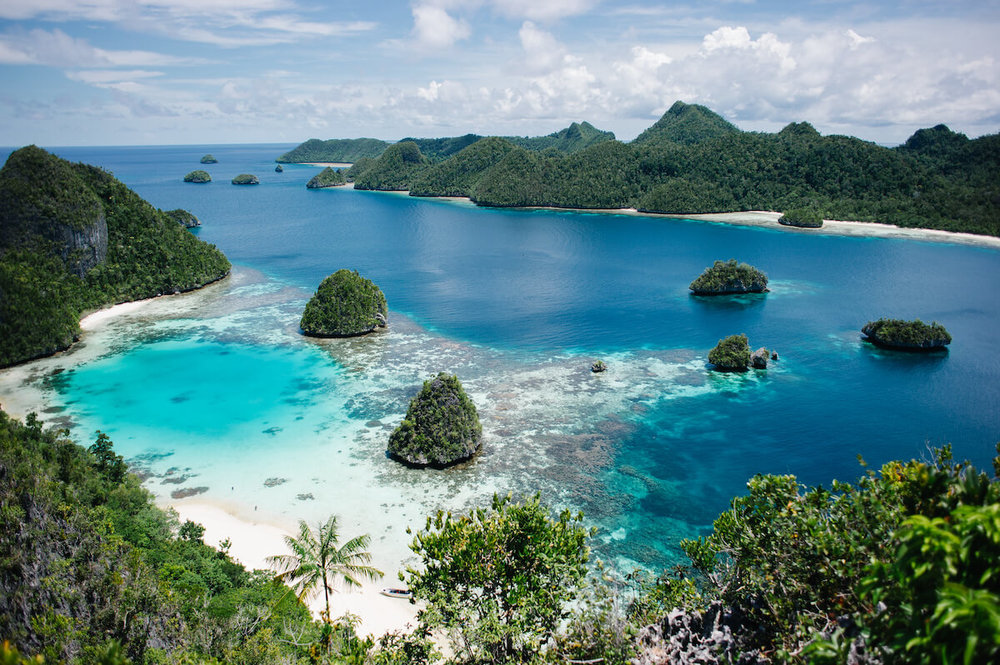
\includegraphics[width=\textwidth]{rajaampat.eps}
      \caption{ラジャ・アンパット}
    \end{subfigure}
    \hfill
    \begin{subfigure}[b]{0.3\textwidth}
      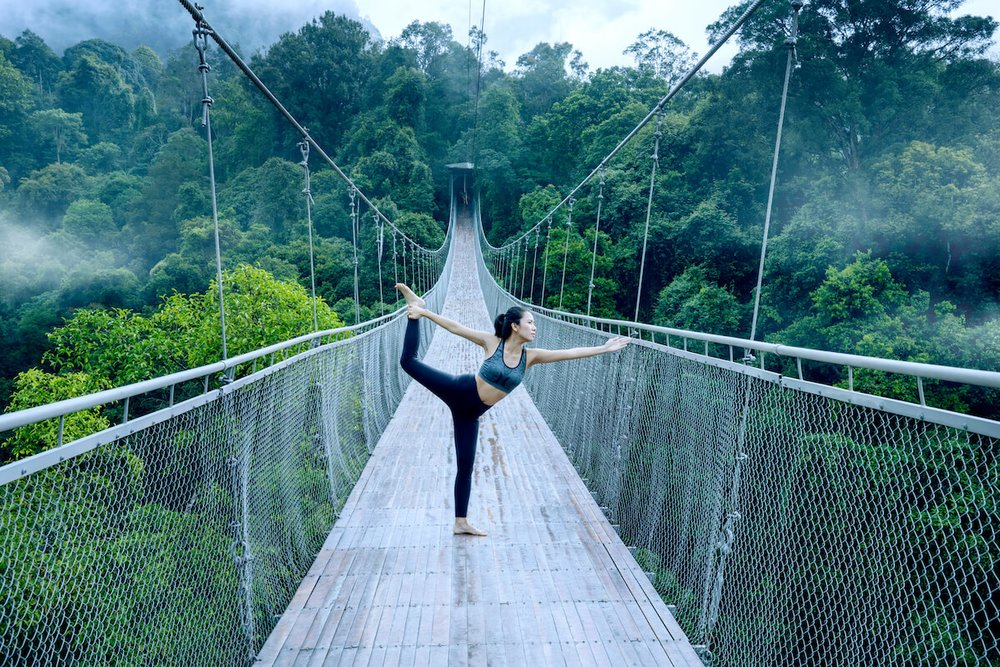
\includegraphics[width=\textwidth]{situgunung.eps}
      \caption{シトゥグヌン}
    \end{subfigure}
    \hfill
    \begin{subfigure}[b]{0.3\textwidth}
      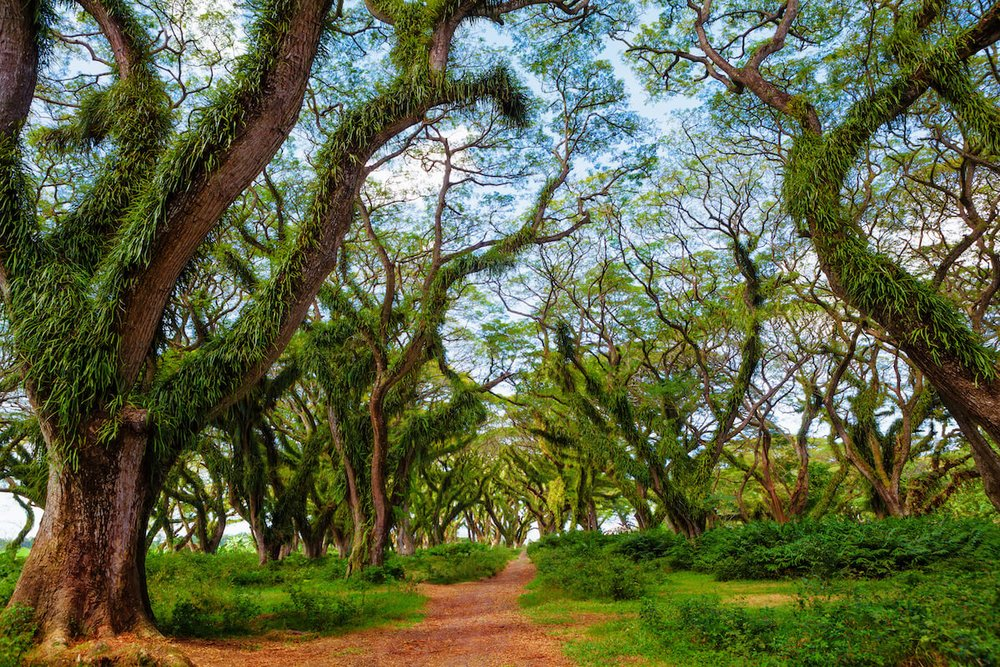
\includegraphics[width=\textwidth]{djawatan.eps}
      \caption{ふーたん・デ・ジャワタン}
    \end{subfigure}
    \caption{インドネシアにある観光地}\label{tourism}
  \end{figure}
  自然災害の危険性があるにもかかわらず, インドネシアは美しい自然にも恵まれています. インドネシアで最も人気のある島の一つはバリ島です. しかし, パプア島のラジャ・アンパット, スカブミのシトゥグヌン, バニュワンギのフータン・デ・ジャワタンなど, 図\ref{tourism}のように, 他にも美しい場所がたくさんあります\cite{klook2023pemandangan}.
  

  \bibliographystyle{plain}
  \bibliography{citations}
\end{document}